\documentclass{article}
\usepackage{titling}
\usepackage{lipsum}
\usepackage{amsmath}
\usepackage{listings}
\usepackage{graphicx}
\usepackage{subcaption}
\usepackage{pgfplots}
\usepgfplotslibrary{statistics}



\begin{document}
\noindent
\begin{minipage}[t]{0.6\textwidth}
    \begin{flushleft}
        \LARGE\textbf{Math 343 - Homework 2} \\
        \vspace{6pt} % add 6pt of vertical space
        \hrule width 10cm
        \vspace{12pt}
        \large\textbf{Preston Duffield} \\
        \large Western Washington University \\
        % \today
        April 14, 2023
        \vspace{24pt}
    \end{flushleft}
\end{minipage}

\section*{Question 1}

Data with a rightward skew would produce a normal probability plot with a positive curvature.
Below is an example of a histogram that would produce a positively curved normal probability plot. \\


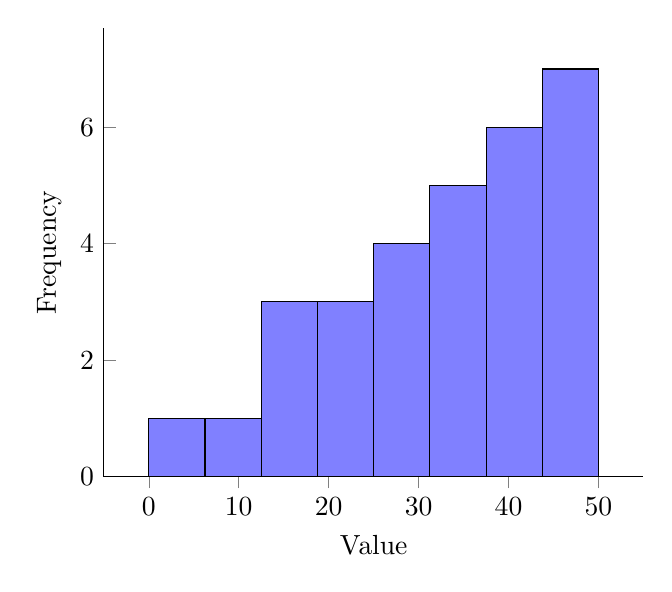
\begin{tikzpicture}
  \begin{axis}[
      ybar,
      ylabel={Frequency},
      xlabel={Value},
      ymin=0,
      axis lines*=left,
      % xtick=data,
      % nodes near coords,
      % nodes near coords align={vertical},
  ]
  \addplot[
      fill=blue!50,
      hist={
          bins=8,
          data min=0,
          data max=50,
      },
  ] table[row sep=\\,y index=0] {
      data \\
      36 \\ 30 \\ 25 \\ 40 \\ 20 \\ 6 \\
      35 \\ 9 \\ 50 \\ 24 \\ 40 \\
      15 \\ 16 \\ 17 \\ 50 \\ 21 \\
      25 \\ 50 \\ 40 \\ 30 \\ 32 \\
      35 \\ 36 \\ 38 \\ 40 \\ 42 \\
      45 \\ 46 \\ 48 \\ 50 \\
  };
  \end{axis}
  \end{tikzpicture}

\section*{Question 2}

\section*{Question 3}

\section*{Question 4}

\section*{Question 5}

\section*{Question 6}

\section*{Question 7}

\section*{Question 8}

\end{document}
